\documentclass{article}
\usepackage{tikz}
\usepackage{forloop}
\usetikzlibrary{shapes.geometric, arrows}
\begin{document}
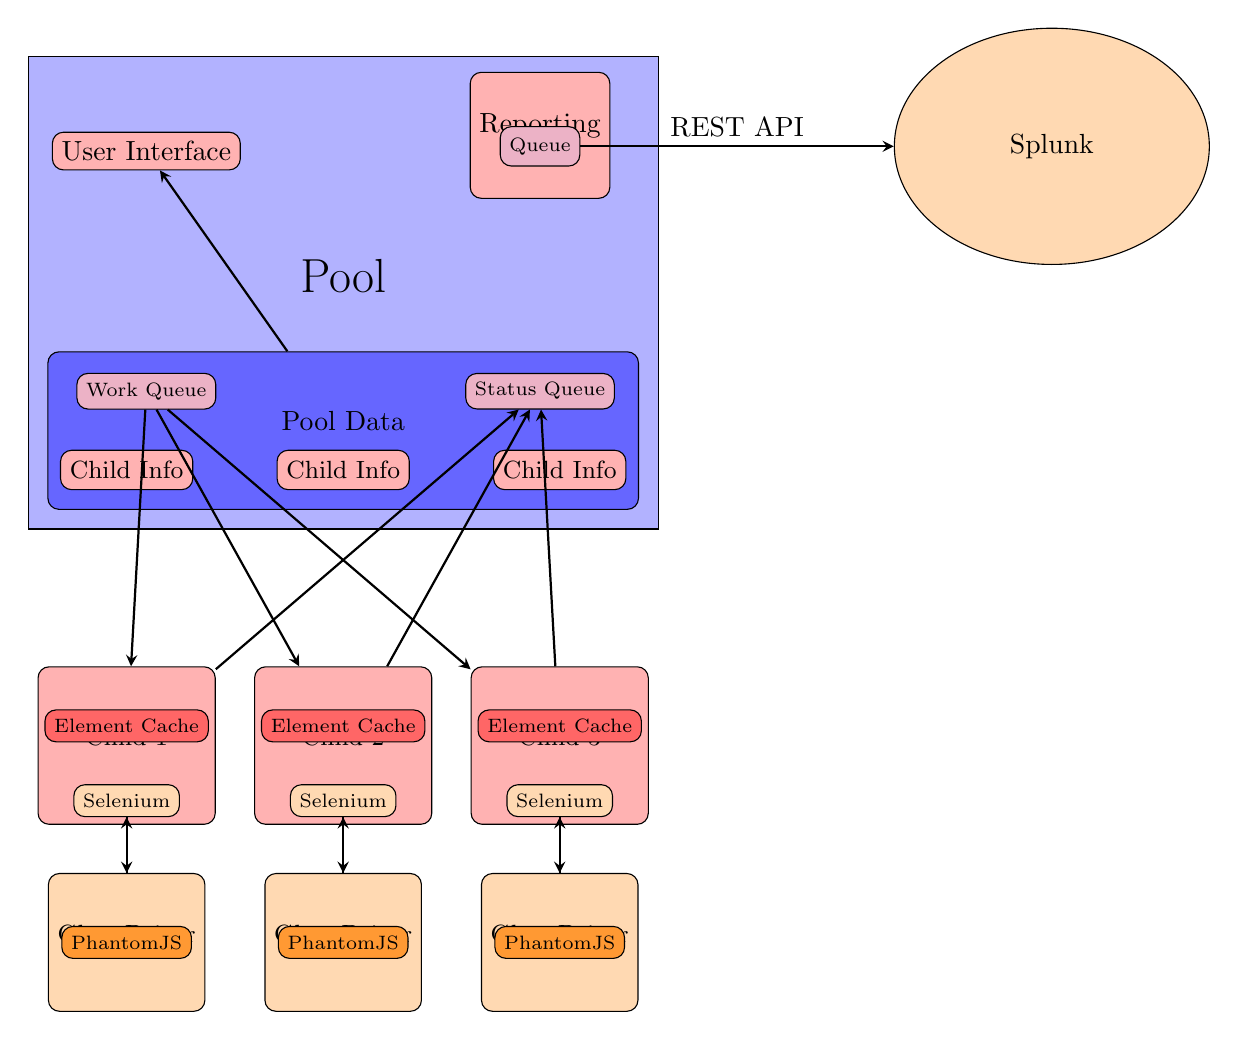
\begin{tikzpicture}

  \tikzstyle{startstop} = [rectangle, rounded corners, minimum width=3cm, minimum height=1cm,text centered, draw=black, fill=red!30]
  \tikzstyle{process} = [rectangle, minimum width=3cm, minimum height=1cm, text centered, draw=black, fill=orange!30]
  \tikzstyle{decision} = [diamond, minimum width=3cm, minimum height=1cm, text centered, draw=black, fill=green!30]

  \tikzstyle{external} = [rectangle, rounded corners, text centered, draw=black, fill=orange!30]
  \tikzstyle{internal} = [rectangle, rounded corners, text centered, draw=black, fill=red!30]
  \tikzstyle{child}    = [internal, minimum height=2cm, minimum width=2.25cm, text height=-1.25cm]
  \tikzstyle{childdata}    = [internal, minimum height=0.5cm, minimum width=0.5cm]
  \tikzstyle{q} = [internal, fill=purple!30]

  \tikzstyle{arrow} = [thick,->,>=stealth]

  \node (pool) [rectangle, minimum width=8cm, minimum height=6cm, text height=-4.5cm, text centered, draw=black, fill=blue!30] {\LARGE Pool};
  %\node (python)  [external, fill=green!30, yshift=1.75cm, xshift=-2.5cm] {Python 2.7}; 
  \node (report)  [internal, minimum height=1.6cm, yshift=2cm, xshift=2.5cm, text height=-0.75cm] {Reporting}; 
  \node (reportqueue) [q, minimum height=0.5cm, below of=report, yshift=0.86cm] {\scriptsize Queue};

  \node (ui) [internal, above of=pool, yshift=0.8cm, xshift=-2.5cm] {User Interface};

  \node (splunk) [external, right of=pool, ellipse, xshift=8cm, yshift=1.86cm, minimum width=4cm, minimum height=3cm] {Splunk};
  \draw [arrow] (reportqueue) -- node[anchor=south] {REST API} (splunk);

  \node (pooldata) [internal, fill=blue!60, minimum width=7.5cm, minimum height=2cm, text height=-1cm, yshift=-1.75cm] { Pool Data };
  
  \draw [arrow] (pooldata) -- (ui);
  
  \node (workqueue) [q, below of=pooldata, yshift=1.5cm, xshift=-2.5cm] {\scriptsize Work Queue};
  \node (statusqueue) [q, below of=pooldata, yshift=1.5cm, xshift=2.5cm] {\scriptsize Status Queue};

  \node (child1data)  [childdata, below of=pool, xshift=-2.75cm, yshift=-1.25cm ] {\small Child Info};
  \node (child2data)  [childdata, below of=pool, yshift=-1.25cm ] {\small Child Info};
  \node (child3data)  [childdata, below of=pool, xshift=2.75cm, yshift=-1.25cm ] {\small Child Info};

  \newcounter{cnt}
  \forloop[1]{cnt}{1}{\value{cnt} < 4}{%
    \node (child\arabic{cnt})         [child, below of=child\arabic{cnt}data, yshift=-2.5cm] {\small Child \arabic{cnt}};
    \node (child\arabic{cnt}cache)    [internal, fill=red!60, below of=child\arabic{cnt}, yshift=1.25cm] {\scriptsize Element Cache};
    \node (child\arabic{cnt}selenium) [external, below of=child\arabic{cnt}, yshift=0.3cm] {\scriptsize Selenium};

    %\draw [arrow] (child\arabic{cnt}data) -- (child\arabic{cnt});
    \draw [arrow] (child\arabic{cnt}) -- (statusqueue);
    \draw [arrow] (workqueue) -- (child\arabic{cnt});

    \node (child\arabic{cnt}gd)       [external, below of=child\arabic{cnt}, yshift=-1.5cm, minimum height=1.75cm, minimum width=1.25cm, text height=-0.95cm] {\small GhostDriver}; 
    \node (child\arabic{cnt}pjs)      [external, below of=child\arabic{cnt}gd, yshift=1cm, fill=orange!80] {\scriptsize PhantomJS};

    \draw [arrow] (child\arabic{cnt}selenium) -- (child\arabic{cnt}gd);
    \draw [arrow] (child\arabic{cnt}gd) -- (child\arabic{cnt}selenium);
  }
  

  
















\end{tikzpicture}
\end{document}
